\vsssub
\subsubsection{~$S_{uo}$: Unresolved Obstacles Source Term} \label{sec:UOST}
\vsssub

\opthead{UOST}{\ws}{L. Mentaschi}

Unresolved bathymetric and coastal features, such as cliffs, shoals and small islands, 
are a major source of local error in spectral wave models. 
Their dissipating effects can be accumulated over long distances, and 
neglecting them can compromise the simulation skill on large portions of the domain 
\citep{tol:Waves01a,tol:WaF02,art:Tuomi2014,art:Mentaschi2015a}. 
In \ws\ 
two approaches are available for subscale modelling 
the dissipation due to unresolved obstacles: 
a) a propagation-based approach established for regular grids, described in section 
\ref{sub:num_obst} \citep{tol:OMOD03a, tol:OMOD08a}; and b) the 
Unresolved Obstacles Source Term \citep[UOST,][]{art:Mentaschi2018a,art:Mentaschi2015b}
described here.
In addition to supporting virtually any type of mesh, 
UOST takes into account the directional/spatial layout 
of the unresolved features, which can improve the model skill
with respect to the established approach \citep{art:HMM00,art:Mentaschi2018b}.

UOST relies on the hypothesis that any mesh can be considered as a set of polygons, 
called cells, and that the model estimates the average value of the unknowns 
in each cell. 
Given a cell (let us call it A, figure \ref{fig:UOST}ab) UOST estimates, for each spectral component, 
the effect of a) the unresolved features located in A (Local Dissipation, LD); 
b) the unresolved features located upstream of A, and projecting their shadow on A 
(Shadow Effect, SE). For the estimation of SE, 
an upstream polygon A\textsc{\char13} is defined for each 
cell/spectral component, as the intersection between the joint cells neighboring A 
(cells B, C and D in figure \ref{fig:UOST}ab), and the flux upstream of A. 
For each cell or upstream polygon, and for each spectral component, 
two different transparency coefficients are estimated. 
1) The overall transparency coefficient $\alpha$; and 
2) a layout-dependent transparency $\beta$, defined as the average transparency 
of cell sections starting from the cell upstream side. 

The source term can be expressed as:

\begin{equation}
S_{uo} = S_{ld} + S_{se}\ ,
\end{equation}

\begin{equation}
S_{ld} = - \psi_{ld}(\mathbf{k}) \frac{1 - \beta_l(\mathbf{k})}{\beta_l(\mathbf{k})} \frac{c_g(\mathbf{k})}{\Delta L} N \ ,
\end{equation}

\begin{equation}
S_{se} = - \psi_{se}(\mathbf{k}) \bigg[ \frac{\beta_u(\mathbf{k})}{\alpha_u(\mathbf{k})} - 1 \bigg] \frac{c_g(\mathbf{k})}{\Delta L} N \ ,
\end{equation}

where $S_{ld}$ and $S_{se}$ are the local dissipation and the shadow effect,
$N$ is the spectral density, 
$\mathbf{k}$ is the wave vector, 
$c_g$ is the group velocity, $\Delta L$ is the path length of the spectral component 
in the cell, and the $\psi$ factors model the reduction of the dissipation in presence of
local wave growth. 
The subscripts l and u of $\alpha$ and $\beta$ indicate that these coefficients 
can be referred, respectively, to the cell and to the upstream polygon.
For a more detailed explanation on the theoretical framework of UOST, 
the reader is referred to
\citep{art:Mentaschi2015b, art:Mentaschi2018a}.


\begin{figure} \begin{center}
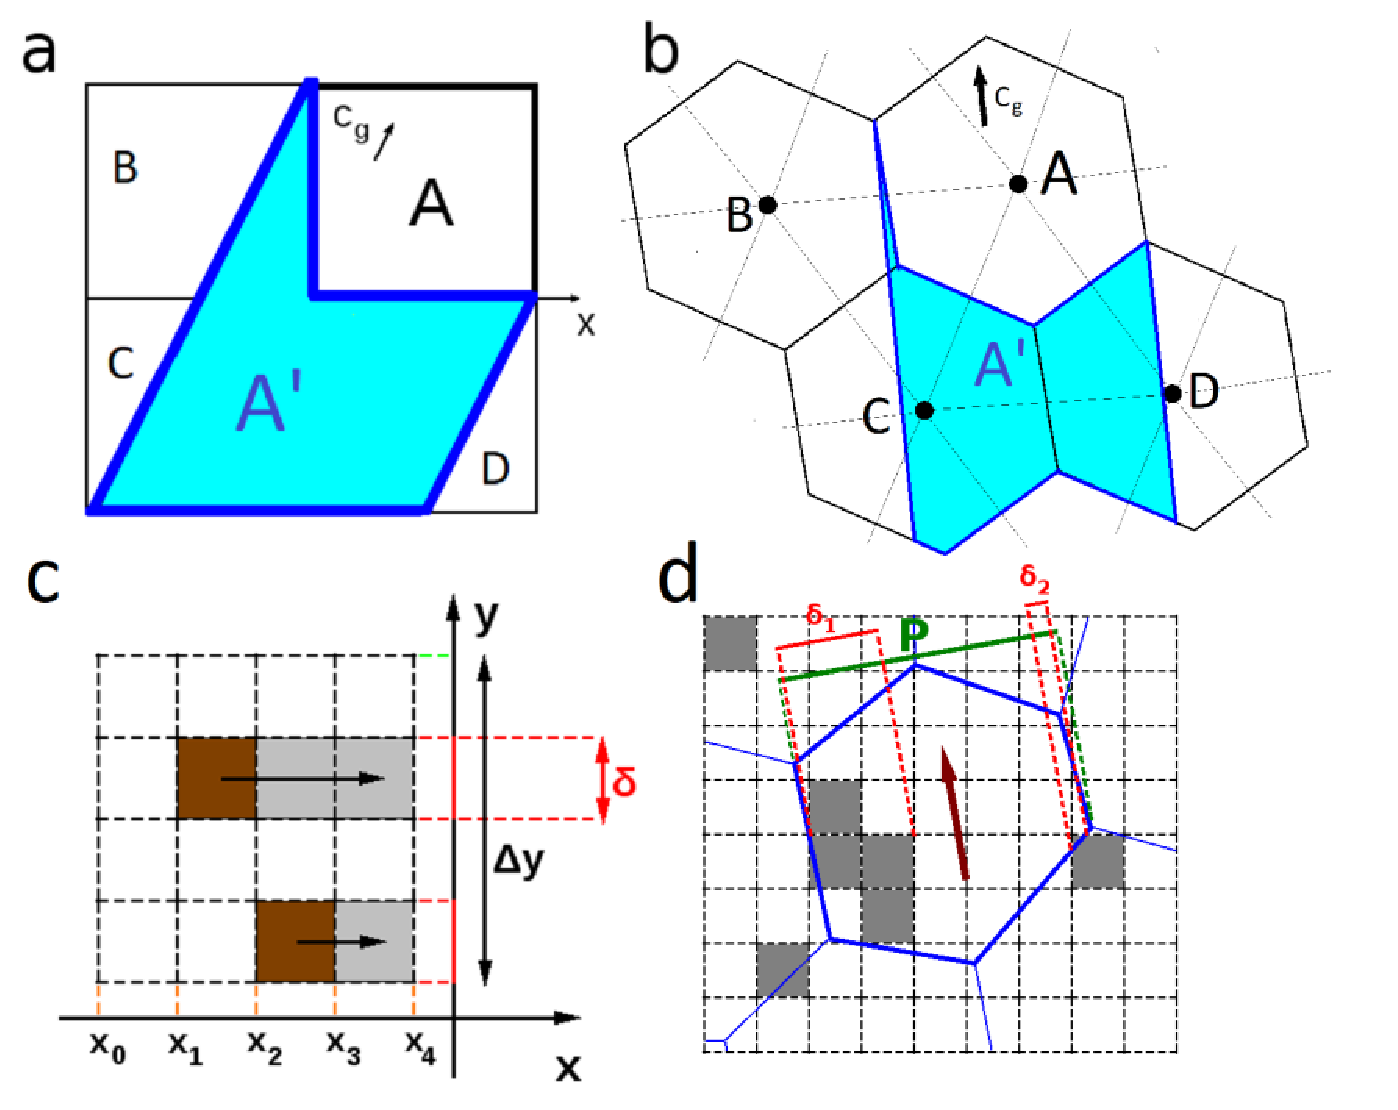
\epsfig{file=./eqs/UOST.eps,angle=0,width=4in}
\caption{
a: a square cell (A) and its upstream polygon 
(A\textsc{\char13}, delimited by blue line, in light blue color) for a spectral 
component propagating with group velocity $c_g$. 
The joint BCD polygon represents the neighborhood polygon. 
b: same as a, but for a triangular mesh (the hexagons approximate the median dual cells). 
c: Computation of $\alpha$ and $\beta$ for a square cell, $N_s=4$, 
and a spectral component propagating along the x axis. 
d: Like c, but for a hexagonal cell and for a tilted spectral component. 
In panel d he gray squares represent unresolved obstacles. 
}
\label{fig:UOST} \botline
\end{center}
\end{figure}


\textbf{Automatic generation of mesh parameters.} 
An open-source python package (alphaBetaLab, https://github.com/menta78/alphaBetaLab) 
was developed
for the automatic estimation, from real-world bathymetry, of the upstream polygons, 
of the transparency coefficients
$\alpha_l$, $\beta_l$, $\alpha_u$, $\beta_u$,
and of the other parameters needed by UOST.
alphaBetaLab considers the cells as free polygons, and estimates the transparency coefficients
from the cross section of the unresolved obstacles versus the incident spectral component 
(figure \ref{fig:UOST}cd).
This involves, that it can be applied to any type of mesh, 
including unstructured triangular and SMC meshes 
(as of August 2018 only regular and triangular meshes are handled, 
but support for SMC meshes 
will be soon added). 
We need to mention that while UOST would be able to modulate the energy dissipation 
with the spectral frequency, only the direction is currently considered in alphaBetaLab.
For more details on the algorithms implemented in alphaBetaLab, 
the user is referred to \cite{art:Mentaschi2018a}. 
\cite{art:Mentaschi2018c} provides the documentation of the software and of its architecture,
along with use guidance and illustrative examples. 

\textbf{Time step settings.} 
In \ws\ the source terms are applied at the end of each global time step.
Therefore, to work properly on a given cell, 
UOST needs a global time step lower
or equal to the critical CFL time step of the cell, 
i.e., the amount of time needed by the fastest spectral component to entirely cross the cell.
Otherwise, part of the energy will leak through the cell without being blocked \citep{art:Mentaschi2018a}.

In unstructured grids with cells of very different sizes, the application of UOST to 
all the cells, including the smallest ones, may come with an excedingly small global time step
that would affect the economy of the model. 
To avoid this problem the user can set alphaBetaLab in order to
neglect cells smaller than a user-defined threshold, and then set in \ws\
a global time step equal to the critical CFL time step related with that threshold 
\citep{art:Mentaschi2018c}.


\begin{table} \begin{center}
\begin{tabular}{|l|p{4cm}|c|} \hline \hline
Namelist parameter    &  Description           & default value \\
\hline
  UOSTFILELOCAL &  Local $\alpha$/$\beta$ input file path   &  obstructions\_local.\textit{gridname}.in    \\ \hline
  UOSTFILESHADOW &  Shadow $\alpha$/$\beta$ input file path   & obstructions\_shadow.\textit{gridname}.in   \\ \hline
  UOSTFACTORLOCAL &  Calibration factor for local transparencies  &  1   \\ \hline
  UOSTFACTORSHADOW &  Calibration factor for shadow transparencies  &  1  \\
\hline
\end{tabular} \end{center}
\caption{UOST parameters, their description and default values. } \label{tab:UOST}
\botline
\end{table}

